%!TEX program = xelatex
% This is a small sample LaTeX input file (Version of 10 April 1994)
%
% Use this file as a model for making your own LaTeX input file.
% Everything to the right of a  %  is a remark to you and is ignored by LaTeX.
 
% The Local Guide tells how to run LaTeX.
 
% WARNING!  Do not type any of the following 10 characters except as directed:
%                &   $   #   %   _   {   }   ^   ~   \   
 
%\documentclass{article}        % Your input file must contain these two lines 
\documentclass[12pt, a4paper, oneside]{ctexart}
\usepackage{xeCJK}

\usepackage{indentfirst, abstract, appendix} %首行缩进
\usepackage{graphicx} %插入图片
\usepackage{amsmath, amssymb, geometry} 
\usepackage{listings, xcolor} %代码高亮
\graphicspath{{../graphics/}}
\linespread{1.2}
\geometry{left=2.5cm, right=2.5cm, top=2.5cm, bottom=2.5cm}
\title{\textbf{神经网络的数学推导和Python实现}}
\author{赵新锋}
\date{\today}
\renewcommand{\abstractname}{\Large\textbf{摘要}}
\pagestyle{plain}

\lstset{ %
language=Python,                % the language of the code
basicstyle=\footnotesize,           % the size of the fonts that are used for the code
%numbers=left,                   % where to put the line-numbers
%numberstyle=\tiny\color{gray},  % the style that is used for the line-numbers
stepnumber=2,                   % the step between two line-numbers. If it's 1, each line 
                                % will be numbered
numbersep=5pt,                  % how far the line-numbers are from the code
backgroundcolor=\color{white},      % choose the background color. You must add \usepackage{color}
showspaces=false,               % show spaces adding particular underscores
showstringspaces=false,         % underline spaces within strings
showtabs=false,                 % show tabs within strings adding particular underscores
frame=single,                   % adds a frame around the code
rulecolor=\color{black},        % if not set, the frame-color may be changed on line-breaks within not-black text (e.g. commens (green here))
tabsize=2,                      % sets default tabsize to 2 spaces
captionpos=b,                   % sets the caption-position to bottom
breaklines=true,                % sets automatic line breaking
breakatwhitespace=false,        % sets if automatic breaks should only happen at whitespace
title=\lstname,                 % show the filename of files included with \lstinputlisting;
                                % also try caption instead of title
keywordstyle=\color{blue},          % keyword style
commentstyle=\it\color[RGB]{0,96,96},                % 设置代码注释的格式
stringstyle=\rmfamily\slshape\color[RGB]{128,0,0},         % string literal style
escapeinside={\%*}{*)},            % if you want to add LaTeX within your code
morekeywords={*,...}               % if you want to add more keywords to the set
}
\begin{document}               % plus the \end{document} command at the end.
\maketitle

\setcounter{page}{0}
\maketitle
\thispagestyle{empty}

\begin{abstract}
神经网络可以说是目前人工智能算法中应用最为广泛的算法之一,相比Linear regression 、
logistics regression、decision tree等机器学习算法等会复杂不少,变化也很多。本文从向量矩阵
的角度去理解BP神经网络的数学原理,这个过程会显得更加清晰、简洁。我们以最经典的神经网络三层
网络二分类模型为例,逐步推导数学公式。
\par\textbf{关键词:}神经网络; 梯度下降; 反向传播; 矩阵运算; 矩阵求导;numpy;sklearn. 
\end{abstract}

\newpage
\pagenumbering{Roman}
\setcounter{page}{1}
\tableofcontents
\newpage
\setcounter{page}{1}
\pagenumbering{arabic}


\newpage
\section{数学推导与python实现}

\subsection{符号定义}
三层网络简单说明如下:
\begin{itemize}
    \item 输入层,不做处理,只是输入数据
    \item 隐藏层,单元数为 $ n_h $ 我们就以RELU为激活函数,另外一个常用的是sigmoid,我们把激活函数封装成一个类,可以随时替换 
    \item 输出层为一个单元,由于是二分类,我们就用sigmoid拟合对应类1的概率
\end{itemize}
\begin{figure}[htbp]
    \centering
    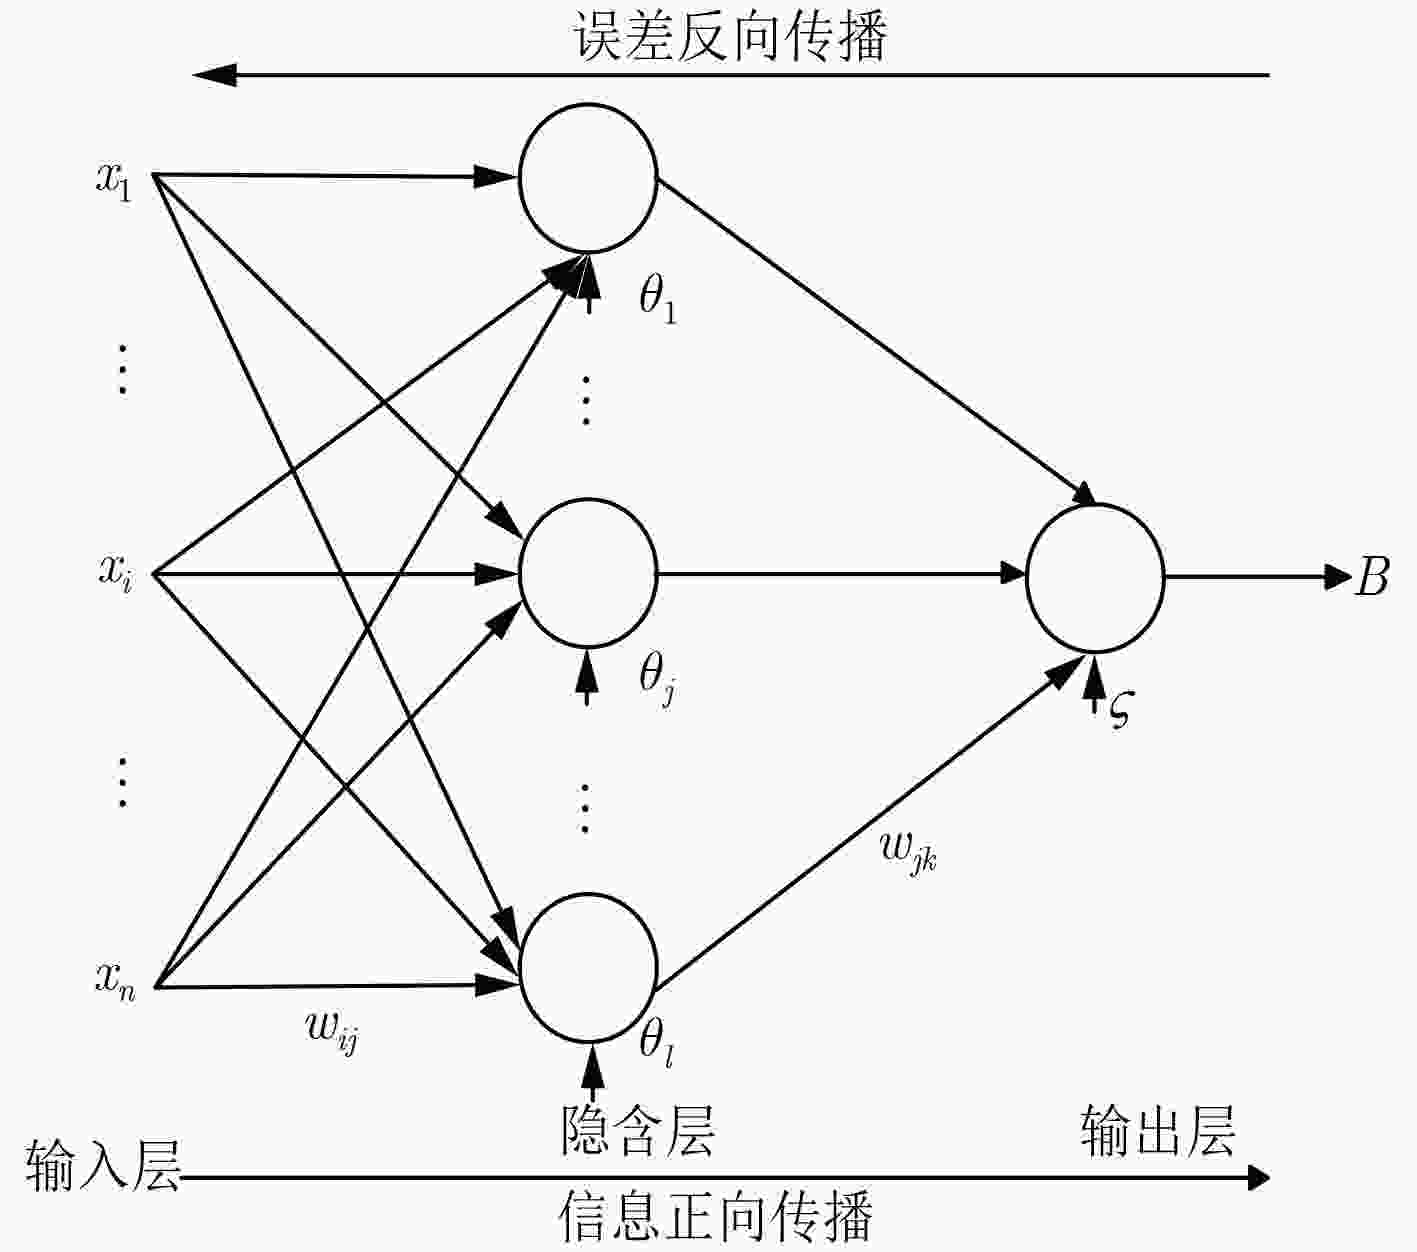
\includegraphics[width=14cm]{bpnn.png}
    \caption{神经网络示意图}\label{fig1}
\end{figure}


\begin{itemize}
\item $X$ 表示输入样本向量矩阵,$Y$表示样本集的期望输出标记(有可能是0/1标记的向量,有可能是onehot的矩阵),本文示例由于是二分类,那么Y的每个元素要么是0要么是1,$Y$是m个元素的向量,但是在运算中为了通用将其转换为$m\times 1$的矩阵。
\item $m$为样本数量,$n$为样本向量的维度。
\item 激活函数用$f$表示,隐藏层激活函数$f_h$使用RELU函数:$f_h(x) = max(0, x)$,输出层$f_o$为sigmoid函数,输出为1类的概率$f_o(x) = \frac{1}{1+exp(-x)}$
\item 隐藏层输出为$Y_h$,输出层的输出为$Y_o$
\item 隐藏层单元的参数为$w_h$, $N_h$个隐藏层单元的参数矩阵为$W_h$,输出层单元的参数为$w_o$,$N_o$个输出层单元的参数矩阵为$W_o$。
\item 虽然本文使用二分类即输出单元为1个,但是仍然使用矩阵$Yo $ 和 $ W_o$表示,从而使得算法是通用的,改成onehot+softmax方式的多分类,也是适用的。
\item 从输入到输出的公式:$Y_o = f_o(f_h(X \cdot W_h) \cdot Wo)$
\item 注:这里的线性变换$X \cdot W_h$并没有使用偏置,通过在$X$增加一个全1的列,达到同样的效果。
\end{itemize}


\subsection{forward公式推导}
单个样本的运算过程表示如下:
\begin{align*}
    x_{hj} &= x_i \cdot w_{hj} 			\\
	y_{hj} &= f_h(x_{hj}) 				\\
	x_o &= y_{hj} \cdot w_{o} 			\\
	y_{o} &= f_o(x_o) 					\\
\end{align*}

批量样本利用矩阵表示运算过程如下:
\begin{align}
	X_h  &= X \cdot W_h 							\nonumber\\
	Y_h  &= f_h(X_h) 								\nonumber\\
	X_o  &= Y_h \cdot W_o 							\nonumber\\
    Y_o  &= f_o(X_o) 								\nonumber\\
    	 &= f_o(Y_h \cdot W_o) 					    \nonumber\\
    	 &= f_o(f_h(X_h) \cdot W_o) 				\nonumber\\
         &= f_o(f_h(X \cdot W_h) \cdot Wo)          \label{eq1}
\end{align}

其中 \eqref{eq1} 式即为信息正向传导的向量化公式相应的python代码实现:

\begin{lstlisting}
#forward
Lh = np.dot(X, Wh)
Yh = funcActivation.cal(Lh) #隐藏层输出
Yh = np.insert(Yh, np.shape(Yh)[1], values=np.ones(m), axis=1)
Lo = np.dot(Yh, Wo)
Yo = funcOut.cal(Lo)
\end{lstlisting}

其中 funcActivation 为隐藏层激活函数的封装,这里使用的Relu,funcOut为输出层激活函数的封装,使用的是sigmoid。
\begin{lstlisting}
class ReLU:
    def cal(self, z):
        return np.clip(z, 0, np.inf)
    def grad(self, x):
        return (x > 0).astype(int)
class Sigmoid:
    def cal(self, z):
        return 1 / (1 + np.exp(-z))
    def grad(self, x):
        z = self.cal(x)
        return z*(1-z)
\end{lstlisting}

\subsection{损失函数}
最常用的有Mean Square Error均方差损失函数,用于分类的Cross Entropy等。本文以经典的MSE为例。如下 \eqref{eq2} 式是MSE损失函数的向量化表示。
\begin{align}
	e 	&= \frac{1}{2m}\sum_{i=1}^{m} (y_{oi} - y_i)^2 				\nonumber\\
		&= \frac{1}{2m}(Y_o - Y)^T \cdot (Y_o - Y)                  \label{eq2}	
\end{align}


\subsection{误差反向传播}

我们目的是最小化损失函数,通常使用梯度下降法,逐渐逼近最小极值点。需要逐渐求解参数主要是两个:
$W_h$ 和  $W_o$ ,下面分别计算对应损失函数的偏导数。
\begin{align}
\mathrm{d}e &= \frac{1}{2m}tr((\mathrm{d}Y_o)^T \cdot (Y_o - Y)  +  (Y_o - Y)^T \cdot \mathrm{d}Y_o)  \nonumber\\
	&= \frac{1}{2m}tr((\mathrm{d}Y_o)^T \cdot (Y_o - Y))  +  \frac{1}{2m}tr((Y_o - Y)^T \cdot \mathrm{d}Y_o)  \nonumber\\
	&= \frac{1}{2m}tr(\mathrm{d}Y_o \cdot (Y_o - Y)^T)  +  \frac{1}{2m}tr((Y_o - Y)^T \cdot \mathrm{d}Y_o)  \nonumber\\
	&= \frac{1}{m}tr((Y_o - Y)^T \cdot \mathrm{d}Y_o) \label{eq3} \\
	&= \frac{1}{m}tr((Y_o - Y)^T \cdot (f_o^{'}(X_o) \odot \mathrm{d}X_o)) \label{eq4} \\
	&= \frac{1}{m}tr(((Y_o - Y) \odot f_o^{'}(X_o))^T \cdot \mathrm{d}X_o) \label{eq5} \\
	&= \frac{1}{m}tr(((Y_o - Y) \odot f_o^{'}(X_o))^T \cdot (Y_h \cdot \mathrm{d}W_o + \mathrm{d}Y_h \cdot W_o))  \label{eq6}
\end{align}

其中 \eqref{eq3} 式利用迹$tr(A^T) = tr(A)$ 的性质,所以前后两项一样 \eqref{eq4} 式到
\eqref{eq5} 式利用了迹$tr(A^T \cdot (B \odot C)) = tr((A \odot B)^T \cdot C)$的性质,
其中$\odot$表示矩阵各个元素相乘,对应numpy的multiply。神经网络梯度下降求解参数的时候,是从输出
层到隐藏层逆着计算的,所以称之为“反向传播”,因此首先求对$W_o$的偏导,此时$Y_h$相当于常数,故
\eqref{eq6} 式的$\mathrm{d}Y_h$ 忽略,继续推导:
\begin{align}
\mathrm{d}e &= \frac{1}{m}tr(((Y_o - Y) \odot f_o^{'}(X_o))^T \cdot (Y_h \cdot \mathrm{d}W_o))    \nonumber\\
    &= \frac{1}{m}tr((Y_h^T \cdot ((Y_o - Y) \odot f_o^{'}(X_o)))^T \cdot \mathrm{d}W_o)   \label{eq7} \\
    \frac{\partial e}{\partial W_o} &= \frac{1}{m}Y_h^T \cdot ((Y_o - Y) \odot f_o^{'}(X_o))    \label{eq8}
\end{align}

这里 \eqref{eq7} 式到 \eqref{eq8} 式利用了标量对向量或矩阵微分
$\mathrm{d}f = tr((\frac{\partial f}{\partial x})^T \mathrm{d}x)$ 的性质。对应python实现:
\begin{lstlisting}
delta = np.multiply(self.lossFunc.grad(Yo, Y) , funcOut.grad(Lo))
dO  = np.dot(Xo.T, delta)
\end{lstlisting}

同理继续推导$\frac{\partial e}{\partial W_h}$ :
\begin{align}
\mathrm{d}e &= \frac{1}{m}tr(((Y_o - Y) \odot f_o^{'}(X_o))^T \cdot (\mathrm{d}Y_h \cdot W_o))  \label{eq9} \\
    &= \frac{1}{m}tr(W_o \cdot ((Y_o - Y) \odot f_o^{'}(X_o))^T \cdot \mathrm{d}Y_h ) \nonumber\\
    &= \frac{1}{m}tr(((Y_o - Y) \odot f_o^{'}(X_o) \cdot W_o^T)^T \cdot \mathrm{d}Y_h ) \nonumber\\
    &= \frac{1}{m}tr(((Y_o - Y) \odot f_o^{'}(X_o) \cdot W_o^T)^T \cdot (f_h^{'}(X_h) \odot \mathrm{d}X_h) )  \nonumber\\
    &= \frac{1}{m}tr((((Y_o - Y) \odot f_o^{'}(X_o) \cdot W_o^T) \odot f_h^{'}(X_h))^T \cdot \mathrm{d}(X_h) ) \label{eq10} \\
    &= \frac{1}{m}tr((((Y_o - Y) \odot f_o^{'}(X_o) \cdot W_o^T) \odot f_h^{'}(X_h))^T \cdot \mathrm{d}(X \cdot W_h) ) \nonumber\\
    &= \frac{1}{m}tr((X^T \cdot (((Y_o - Y) \odot f_o^{'}(X_o) \cdot W_o^T) \odot f_h^{'}(X_h)))^T \cdot \mathrm{d}W_h ) \nonumber\\
    \frac{\partial e}{\partial W_h} &= \frac{1}{m}X^T \cdot (((Y_o - Y) \odot f_o^{'}(X_o) \cdot W_o^T) \odot f_h^{'}(X_h))  \label{eq11}
\end{align}

对应的python的实现:
\begin{lstlisting}
delta = np.multiply(self.lossFunc.grad(Yo, Y) , funcOut.grad(Lo))
dH = np.dot(X.T, np.multiply(np.dot(delta, Wo.T[:,:-1]) , funcActivation.grad(Lh)))
\end{lstlisting}
\subsection{梯度下降}
神经网络的学习过程,即最小化损失函数的过程,是通过梯度下降法迭代求解参数的。其中下式的$\eta$
为学习速率。太大可能出现震荡或不收敛,太小可能收敛的太慢。
\begin{align}    
    \frac{\partial e}{\partial W_o} &= \frac{1}{m}Y_h^T \cdot ((Y_o - Y) \odot f_o^{'}(X_o))    \nonumber \\
    \frac{\partial e}{\partial W_h} &= \frac{1}{m}X^T \cdot (((Y_o - Y) \odot f_o^{'}(X_o) \cdot W_o^T) \odot f_h^{'}(X_h))  \nonumber \\
    W_o &= W_o - \eta\frac{\partial e}{\partial W_o} \nonumber \\
    W_h &= W_h - \eta\frac{\partial e}{\partial W_h} \nonumber
\end{align}

\newpage
\section{使用偏置$b$的数学推导}
以上是使用通过$X$ 增加全1的列的方式,省略偏置$b$,下面再推导一下使用偏置的方式。
\subsection{forward公式推导}
单个样本的运算过程表示如下:
\begin{align}    
    x_{hj} &= x_i \cdot w_{hj} + b_{hj} \nonumber\\
    y_{hj} &= f_h(x_{hj})               \nonumber\\
    x_o &= y_{hj} \cdot w_{o} + b_{oj}  \nonumber\\
    y_{o} &= f_o(x_o)                   \nonumber
\end{align}

批量样本利用矩阵表示运算过程如下:
\begin{align}
	X_h  &= X \cdot W_h + B_h 						\nonumber\\
	Y_h  &= f_h(X_h) 								\nonumber\\
	X_o  &= Y_h \cdot W_o + B_o						\nonumber\\
    Y_o  &= f_o(X_o) 								\nonumber\\
    	 &= f_o(Y_h \cdot W_o + B_o) 				\nonumber\\
    	 &= f_o(f_h(X_h + B_h) \cdot W_o + B_o) 	\nonumber\\
         &= f_o(f_h(X \cdot W_h+ B_h) \cdot Wo + B_o) \label{eq12}
\end{align}

\subsection{偏导公式推导}
使用MSE的损失函数,矩阵运算形式的微分运算如下:
\begin{align}
    de &= \frac{1}{m}tr(((Y_o - Y) \odot f_o^{'}(X_o))^T \cdot \mathrm{d}X_o) \nonumber\\
       &= \frac{1}{m}tr(((Y_o - Y) \odot f_o^{'}(X_o))^T \cdot \mathrm{d}(Y_h \cdot W_o + B_o)) \nonumber\\
       &= \frac{1}{m}tr(((Y_o - Y) \odot f_o^{'}(X_o))^T \cdot (\mathrm{d}(Y_h \cdot W_o) + \mathrm{d}B_o)) \nonumber
\end{align}

其中 $\frac{\partial e}{\partial W_o}$ 跟 \eqref{eq8} 式的结果相同,继续推导 
$ \frac{\partial e}{\partial B_o} $ :
\begin{align}
de &= \frac{1}{m}tr(((Y_o - Y) \odot f_o^{'}(X_o))^T \cdot \mathrm{d}B_o) \nonumber\\
\frac{\partial e}{\partial W_o} &= \frac{1}{m}Y_h^T \cdot ((Y_o - Y) \odot f_o^{'}(X_o))    \nonumber\\
    \frac{\partial e}{\partial B_o} &= \frac{1}{m}(Y_o - Y) \odot f_o^{'}(X_o) \nonumber
\end{align}

下面推导$\frac{\partial e}{\partial W_o}$ 和 $ \frac{\partial e}{\partial B_h} $ :
\begin{align}
    de &= \frac{1}{m}tr((((Y_o - Y) \odot f_o^{'}(X_o) \cdot W_o^T) \odot f_h^{'}(X_h))^T \cdot \mathrm{d}(X_h) ) \nonumber \\
    &= \frac{1}{m}tr((((Y_o - Y) \odot f_o^{'}(X_o) \cdot W_o^T) \odot f_h^{'}(X_h))^T \cdot \mathrm{d}(X \cdot W_h + B_h) )  \nonumber
\end{align}

显然 $\frac{\partial e}{\partial W_h}$ 跟 \eqref{eq11} 式的结果相同,继续推导 $ \frac{\partial e}{\partial B_o} $ :
\begin{align}
    de &= \frac{1}{m}tr((((Y_o - Y) \odot f_o^{'}(X_o) \cdot W_o^T) \odot f_h^{'}(X_h))^T \cdot \mathrm{d}(X_h) ) \nonumber \\
    &= \frac{1}{m}tr((((Y_o - Y) \odot f_o^{'}(X_o) \cdot W_o^T) \odot f_h^{'}(X_h))^T \cdot \mathrm{d}B_h )  \nonumber\\    
    \frac{\partial e}{\partial W_h} &= \frac{1}{m}X^T \cdot (((Y_o - Y) \odot f_o^{'}(X_o) \cdot W_o^T) \odot f_h^{'}(X_h))  \nonumber\\
    \frac{\partial e}{\partial B_h} &= \frac{1}{m}((Y_o - Y) \odot f_o^{'}(X_o) \cdot W_o^T) \odot f_h^{'}(X_h) \nonumber
\end{align}
\subsection{梯度下降}
相比不使用偏置的梯度下降,多了两个B参数的梯度下降。
\begin{align}    
    \frac{\partial e}{\partial W_o} &= \frac{1}{m}Y_h^T \cdot ((Y_o - Y) \odot f_o^{'}(X_o))    \nonumber \\
    \frac{\partial e}{\partial B_o} &= \frac{1}{m}(Y_o - Y) \odot f_o^{'}(X_o) \nonumber \\
    \frac{\partial e}{\partial W_h} &= \frac{1}{m}X^T \cdot (((Y_o - Y) \odot f_o^{'}(X_o) \cdot W_o^T) \odot f_h^{'}(X_h))  \nonumber \\
    \frac{\partial e}{\partial B_h} &= \frac{1}{m}((Y_o - Y) \odot f_o^{'}(X_o) \cdot W_o^T) \odot f_h^{'}(X_h) \nonumber \\
    W_o &= W_o - \eta\frac{\partial e}{\partial W_o} \nonumber \\
    W_h &= W_h - \eta\frac{\partial e}{\partial W_h} \nonumber \\
    B_o &= B_o - \eta\frac{\partial e}{\partial B_o} \nonumber \\
    B_h &= B_h - \eta\frac{\partial e}{\partial B_h} \nonumber 
\end{align}


\newpage
\section{总结}

\subsection{多层网络}
本文实现的是基于输入层、隐藏层、输出层经典的三层神经网络架构,在此基础上可以实现更多隐藏层的神经
网络。我们观察 隐藏层的参数基于损失函数的偏导 \eqref{eq11} 式与输出层的 \eqref{eq8} 式区别:
\begin{align}
    \frac{\partial e}{\partial W_h} &= X^T \cdot (\overbrace{\frac{1}{m}((Y_o - Y) \odot f_o^{'}(X_o) \cdot W_o^T)}^{\delta_o} \odot f_h^{'}(X_h)) \nonumber\\
    \frac{\partial e}{\partial W_o} &= Y_h^T \cdot (\overbrace{\frac{1}{m}(Y_o - Y)}^{\delta} \odot f_o^{'}(X_o)) \nonumber
\end{align}
我们观察到规律,$ \frac{\partial e}{\partial W_h}$ 可以分成3项, $X^T$ 项是自己这一层的输入,
$\delta_o$ 为上一层的反馈,第3项 为本层激活函数的导数,同理,$ \frac{\partial e}{\partial W_h}$ 
也可以看出三项,其中 $\delta$ 为损失函数的导数,我们可以把他看成输出层的上一层的反馈值,所以
每层的参数矩阵的偏导可以统一公式为:
\begin{align}
    \frac{\partial e}{\partial W_{i}} = X_i^T \cdot (\delta_{i+1} \odot f_i^{'}(X_i \cdot W_i))  \nonumber
\end{align}

\subsection{Linear regression}
如果把隐藏层去掉,输出层的激活函数也去掉,那么只有一层的神经网络就是多元线性回归。
\begin{align}
    Y = X \cdot w + b \nonumber
\end{align}
\subsection{Logistics regression}
如果把隐藏层去掉,输出层的激活函数使用sigmoid,那么只有一层的神经网络就是就变成了逻辑回归。
\begin{align}
    Y = \frac{1}{1+exp(X \cdot w + b)} \nonumber
\end{align}
\subsection{关于隐藏层数量的选择}
有一些启发式的公式选择隐藏层数量,但是主要还是通过实验选择最恰当的参数,这里可以使用交叉验证的
方式。如将训练样本3/7分割为验证数据集和训练数据集,然后先从少的隐藏层数量开始试,选择在训练
数据集上拟合效果好,同时在验证数据集上同样具有接近准确度的参数作为最终参数结果。



\newpage
\begin{thebibliography}{99}
    \bibitem{b}Ian Goodfellow / Yoshua Bengio / Aaron Courville . \emph{Deep Learning}[M]. 北京:清华大学出版社,2017-08-01.
    \bibitem{b}张贤达. \emph{矩阵分析与应用}[M]. 北京:人民邮电出版社,2013-11-01.
    \bibitem{c}李航. \emph{统计学习方法}[M]. 北京:清华大学出版社,2012-03.
    \bibitem{d}David C. Lay / Steven R. Lay / Judi J. McDonald . \emph{线性代数及其应用}[M]. 北京:机械工业出版社,2018-07.
    \bibitem{e}史蒂文·J. 米勒 . \emph{普林斯顿概率论读本}[M]. 北京:人民邮电出版社,2020-08.
\end{thebibliography}


\newpage
\begin{appendices}
\section{附录使用偏置$b$的python源码}
使用偏置$b$的python源码实现,只使用sklearn库:

\begin{lstlisting}
import numpy as np 
from sklearn import datasets
from sklearn.datasets import load_breast_cancer
from sklearn import preprocessing
import matplotlib.pyplot as plt
from sklearn.metrics import r2_score

dataset = None
DT_FLAG = 1 #1测试预测,2测试回归拟合

if DT_FLAG:
    dataset = load_breast_cancer()
else:
    dataset = datasets.load_boston()

class ReLU:
    def __init__(self):
        return
    def cal(self, z):
        return np.clip(z, 0, np.inf)
    def grad(self, x):
        return (x > 0).astype(int)
class Sigmoid:
    def __init__(self):
        return
    def cal(self, z):
        return 1 / (1 + np.exp(-z))
    def grad(self, x):
        z = self.cal(x)
        return z*(1-z)

class LossMSE:
    def __init__(self):
        return
    def loss(self, y_pred, y):
        return np.sum(np.multiply((y_pred - y) , (y_pred - y))) / 2 /int(y.shape[0]) 
    def grad(self, y_pred, y):
        return (y_pred - y)/y.shape[0]
class LossCrossEntropy:
    def loss(self, y_pred, y):
        eps = np.finfo(float).eps
        cross_entropy = -np.sum(y * np.log(y_pred + eps))
        return cross_entropy
    def grad(self, y_pred, y):
        grad = y_pred - y
        return grad

class LinearOut:#如果用于回归,只是线性输出,不做任何转换,为了可以有统一的结构
    def cal(self, z):
        return z
    def grad(self, x):
        self.gradCache = np.ones(np.shape(x))
        return self.gradCache

class NN:
    def __init__(self):
        self.Wh = None #隐藏层参数w
        self.Wo = None #输出层参数w
        self.numHideUnit = 5
        self.funcActivation = ReLU() #隐藏层激活函数
        if DT_FLAG:
            self.lossFunc = LossMSE()
            self.funcOut = Sigmoid()
        else:
            self.lossFunc = LossMSE()
            self.funcOut = LinearOut()
        return
    def fit(self, X, Y):
        scalerX = preprocessing.StandardScaler().fit(X)#StandardScaler
        Y = Y.reshape(-1, 1)
        X = scalerX.transform(X)
        if not DT_FLAG:
            scalerY = preprocessing.StandardScaler().fit(Y)#MinMaxScaler
            Y = scalerY.transform(Y)

        m, n = np.shape(X)

        funcActivation = self.funcActivation
        funcOut = self.funcOut 
        # 10 1000 0.01 for breat cancer
        numLayerHide = 5
        maxIterTimes = 2000 
        eta  = 0.01
        if DT_FLAG:
            eta  = 10
        else:
            #maxIterTimes = 100000
            eta  = 0.5#eta  = 0.00001
            pass

        outputNodeNum = 1
        Wh = np.random.rand(n, numLayerHide) * 0.01 
        Bh = np.random.rand(numLayerHide) * 0.01 
        Wo = np.random.rand(numLayerHide, outputNodeNum) * 0.01 #Why +1? for reserver b 
        Bo = np.random.rand(outputNodeNum) * 0.01 

        errLog = []
        dO_Old = 0
        dH_Old = 0
        for i in range(maxIterTimes):
            #forward
            Lh = np.dot(X, Wh) + Bh            
            Yh = funcActivation.cal(Lh) #隐藏层输出

            Lo = np.dot(Yh, Wo) + Bo
            Yo = funcOut.cal(Lo)

            loss = self.lossFunc.loss(Yo, Y)
            errLog.append(loss)
            if loss < 0.001:
                break
            
            delta = np.multiply(self.lossFunc.grad(Yo, Y) , funcOut.grad(Lo))

            dBo  = delta
            dWo  = np.dot(Yh.T, dBo)
            
            dBh = np.multiply(np.dot(delta, Wo.T) , funcActivation.grad(Lh))
            dWh = np.dot(X.T, dBh)

            Wo = Wo - eta * dWo
            Wh = Wh - eta * dWh
            Bo = Bo - eta * dBo
            Bh = Bh - eta * dBh
        score = 0
        if DT_FLAG == 0:
            score = r2_score(Yo, Y)
        else:
            score = r2_score((Yo > 0.5).astype(int), Y)
        print('score', score)
        return
if __name__ == '__main__':
    nn = NN()
    print('data', dataset.data.shape)
    nn.fit(dataset.data, dataset.target)
\end{lstlisting}

\end{appendices}
\end{document}                 % The input file ends with this command.

